

\par In order to achieve the ability to predict objects and scenes 
from FMRI images, a predictive model is required. The project was thus 
divided into a few main stages for independent preprocessing of the 
movie description and FMRI images, model building, and prediction
testing.

\centerline{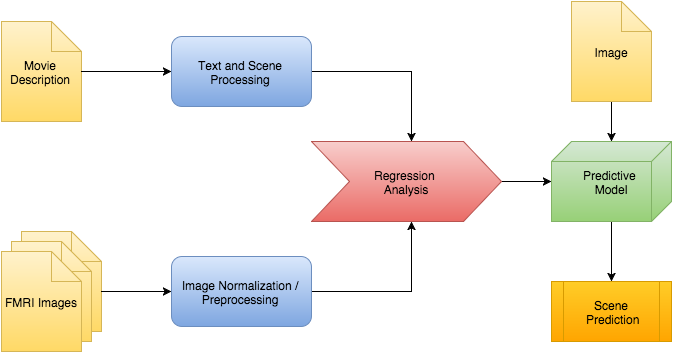
\includegraphics[width=.9\linewidth]{processflow}}

\subsection{Text Preprocessing}
\par As the movie description as provided was in German, we first used Google
Translate to translate the description to English before proceeding with 
any further processing. This decision was made because we believed that 
it

Due to grammatical differences, we decided to
 only keep nouns and verbs, and discarded the adjectives and other words including
 stopwords. Princeton University provides a list of stopwords for text preprocessing.
 Stopwords are the most commonly used natural language words in the English, but have 
 very little meaning. Examples of stop words include "and", "to", and "him". We saved 
 the translated text into a CSV file and parsed in Python. 

\subsection{FMRI Preprocessing}

\subsection{Regression Analysis}

\subsection{Predictive Testing}

